\begin{frame}{}
  Qu'est-ce que Max a fait hier et à quelle heure?
  \begin{columns}
    \column{0.5\textwidth}
      \begin{enumerate}
        \item Max \underline{\uncover<2->{a mangé}} à \underline{\uncover<2->{8h15 du matin}}.
        \item<3-> Max \underline{\uncover<4->{a joué au rugby}} à \underline{\uncover<4->{11h du matin}}.
        \item<5-> Max \underline{\uncover<6->{est sorti de la maison}} à \underline{\uncover<6->{8h du matin}}.
        \item<7-> Max \underline{\uncover<8->{est allé au stade}} à \underline{\uncover<8->{10h du matin}}.
        \item<9-> Max \underline{\uncover<10->{a étudié}} à \underline{\uncover<10->{15h}}.
        \item<11-> Max \underline{\uncover<12->{est rentré}} à \underline{\uncover<12->{1h du matin}}.
        \item<13-> Max et son amie \underline{\uncover<14->{sont allés au ciné}} à \underline{\uncover<14->{8h20 du soir}}.
      \end{enumerate}
    \column{0.5\textwidth}
      \begin{minipage}[c][0.6\textheight]{\linewidth}
        \begin{center}
          \only<1-2>{
            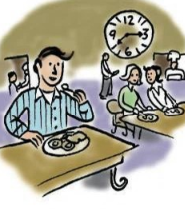
\includegraphics{max_mange.png}
          }
          \only<3-4>{
            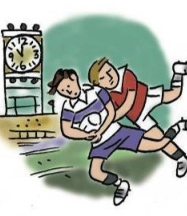
\includegraphics{max_joue.png}
          }
          \only<5-6>{
            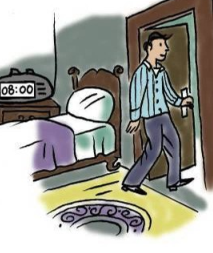
\includegraphics{max_sorti.png}
          }
          \only<7-8>{
            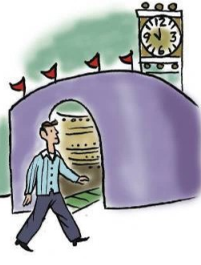
\includegraphics{max_alle.png}
          }
          \only<9-10>{
            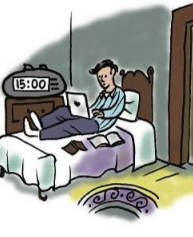
\includegraphics{max_etudie.png}
          }
          \only<11-12>{
            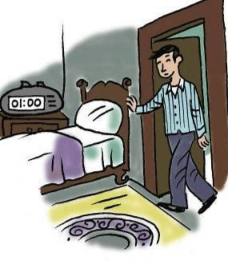
\includegraphics[scale=0.9]{max_rentre.png}
          }
          \only<13->{
            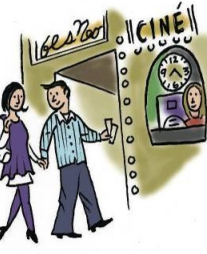
\includegraphics{max_cine.png}
          }
        \end{center}
      \end{minipage}
  \end{columns}
\end{frame}